\begin{frame}\begin{center}
    \LARGE\textbf{Human Capital}
\end{center}\end{frame}
%-------------------------------------------------------------------------------
%-------------------------------------------------------------------------------
\begin{frame}
Human capital is defined as:
\vspace{\baselineskip}

\begin{quote}
The knowledge, skills, competencies and attributes embodied in individuals that facilitate
the creation of personal, social and economic well-being.
\end{quote}\vspace{-0.5pt} \hspace{6cm} - OECD (2001)
\end{frame}
%-------------------------------------------------------------------------------
%-------------------------------------------------------------------------------
\begin{frame}\begin{center}
\LARGE\textit{Basics}
\end{center}\end{frame}
%-------------------------------------------------------------------------------
%-------------------------------------------------------------------------------
\begin{frame}
We study the basic relationship between basic measures of human capital and wages at age thirty-five.
\end{frame}
%-------------------------------------------------------------------------------
%-------------------------------------------------------------------------------
\begin{frame}
\begin{itemize}
\item The \textbf{ Armed Forces Qualifications Test (AFQT)} is a general measure of trainability and a primary criterion of eligibility for service in the armed forces. It has been used extensively as a measure of cognitive skills in the literature (see, e.g., Heckman 1995; Neal and John-
416 Heckman et al. son 1996; Cameron and Heckman 1998; Ellwood and Kane 2000; Cameron
and Heckman 2001; Osborne-Groves 2006).
\end{itemize}
\end{frame}
%-------------------------------------------------------------------------------
%-------------------------------------------------------------------------------
\begin{frame}\begin{figure}[htp]\centering
\caption{AFQT Score}
\scalebox{0.35}{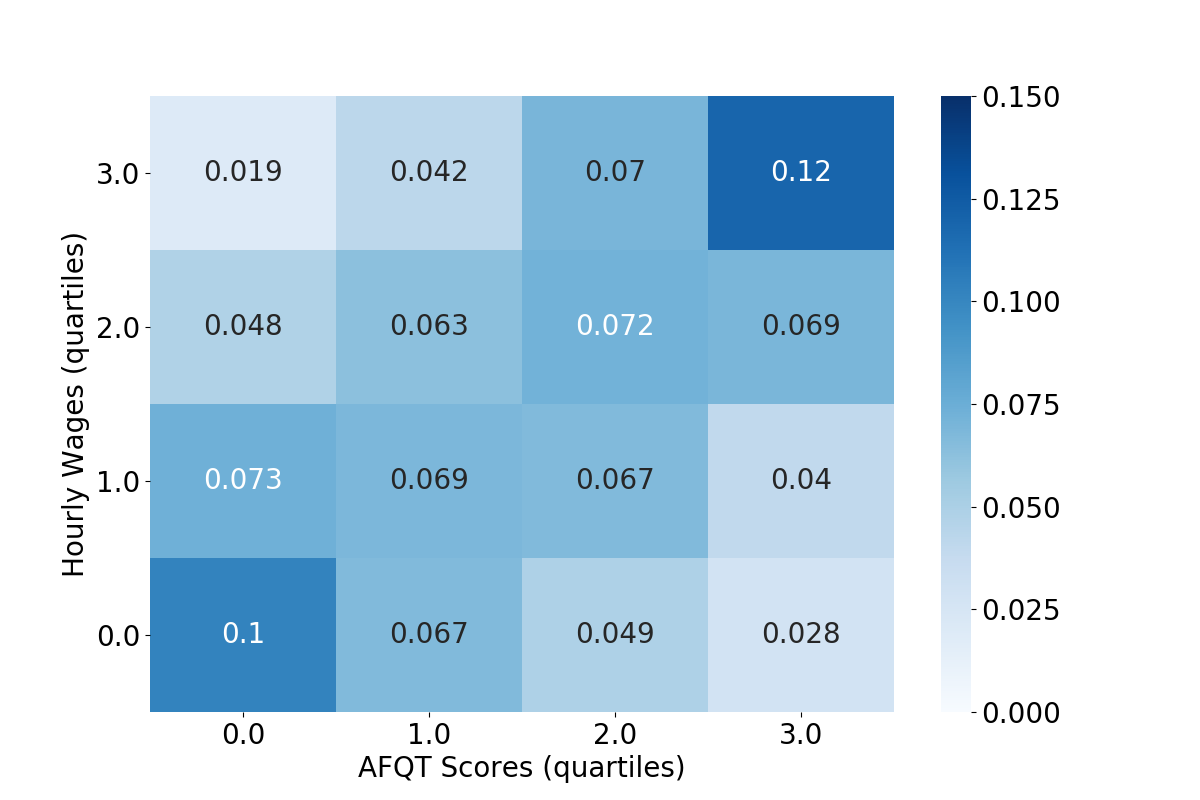
\includegraphics{fig-human-capital-basic-afqt}}
\end{figure}\end{frame}
%-------------------------------------------------------------------------------
%-------------------------------------------------------------------------------
\begin{frame}
\begin{itemize}
\item The \textbf{Rotter scale} measures the degree of control individuals feel they
possess over their life and has been used in previous studies analyzing
the role of noncognitive skills on labor outcomes (Osborne-Groves 2006).
\end{itemize}
\end{frame}
%-------------------------------------------------------------------------------
%-------------------------------------------------------------------------------
\begin{frame}\begin{figure}[htp]\centering
\caption{Rotter Score}
\scalebox{0.35}{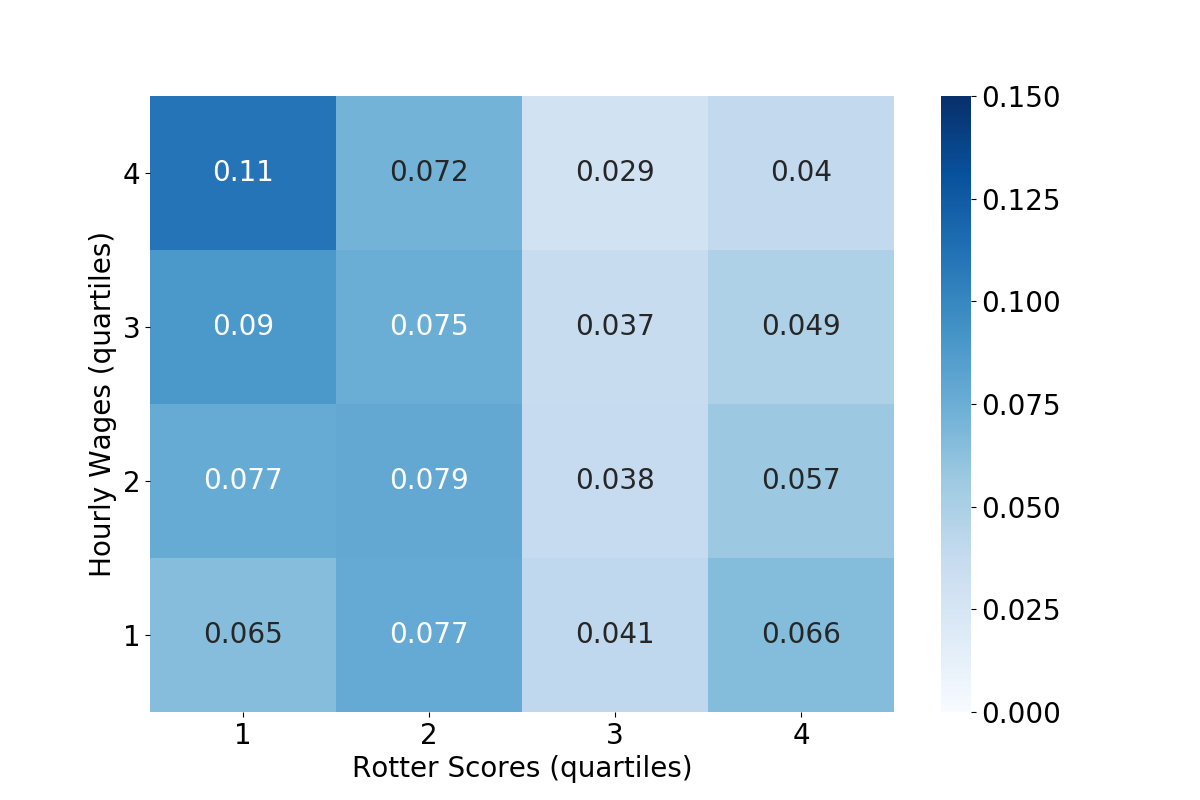
\includegraphics{fig-human-capital-basic-rotter}}
\end{figure}\end{frame}
%-------------------------------------------------------------------------------
%-------------------------------------------------------------------------------
\begin{frame}
\begin{itemize}
\item The \textbf{Rosenberg scale} measures perceptions of self-worth.
\end{itemize}
\end{frame}
%-------------------------------------------------------------------------------
%-------------------------------------------------------------------------------
\begin{frame}\begin{figure}[htp]\centering
\caption{Rosenberg Score}
\scalebox{0.35}{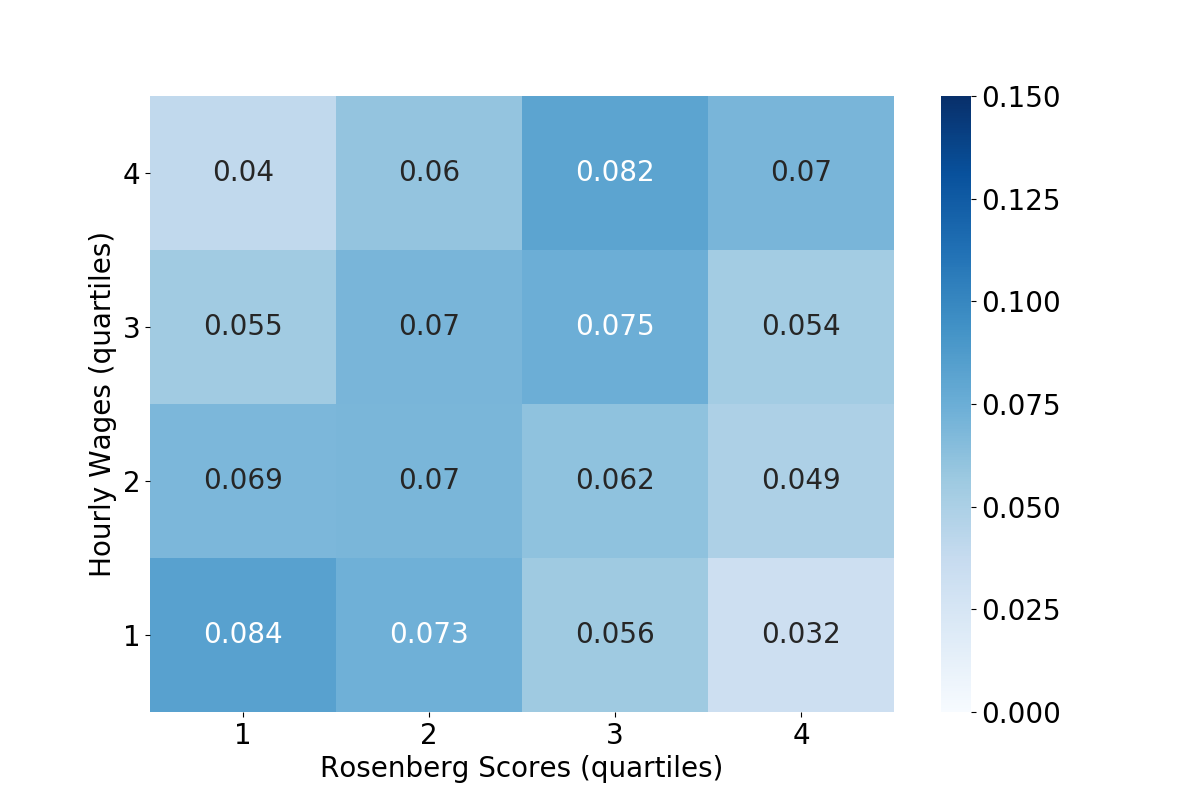
\includegraphics{fig-human-capital-basic-rosenberg}}
\end{figure}\end{frame}
%-------------------------------------------------------------------------------
%-------------------------------------------------------------------------------
\begin{frame}\begin{center}
\LARGE\textit{Racial Differences}
\end{center}\end{frame}
%-------------------------------------------------------------------------------
%-------------------------------------------------------------------------------
\begin{frame}\begin{figure}[htp]\centering
\caption{AFQT Score}
\scalebox{0.35}{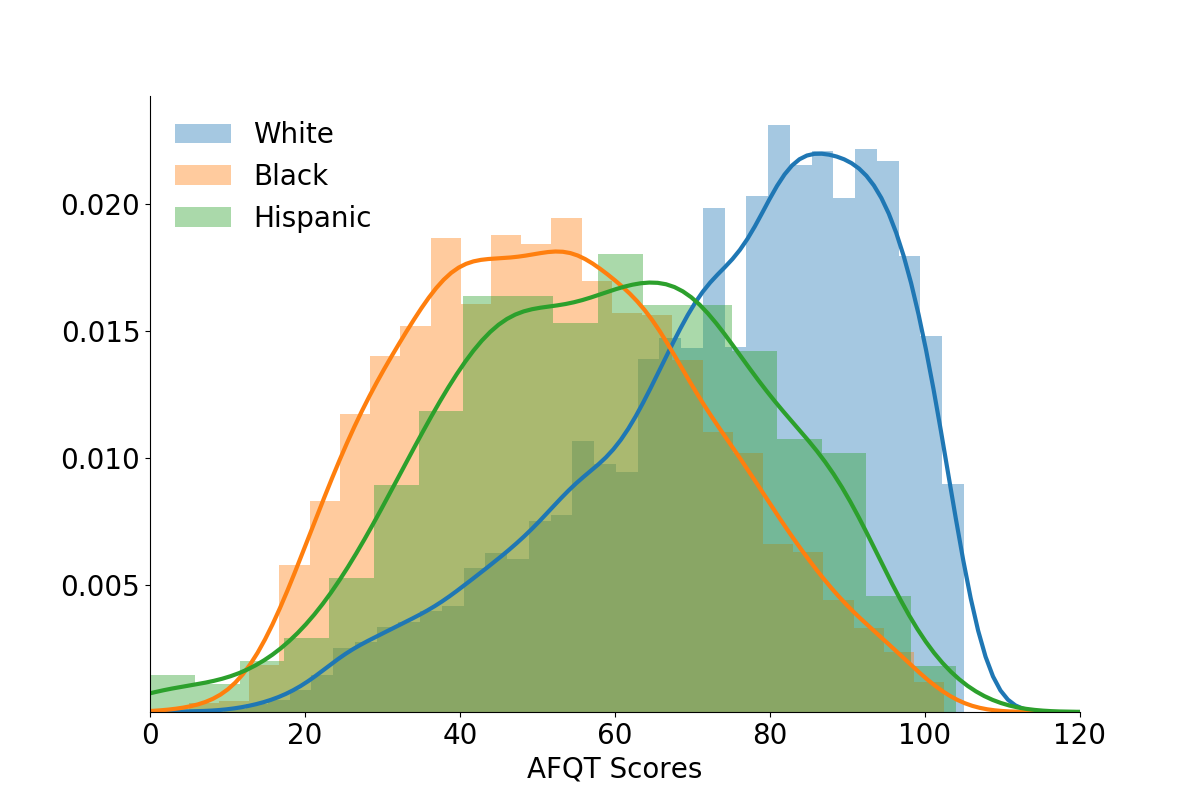
\includegraphics{fig-human-capital-race-afqt}}
\end{figure}\end{frame}
%-------------------------------------------------------------------------------
%-------------------------------------------------------------------------------
\begin{frame}\begin{figure}[htp]\centering
\caption{Rotter Score}
\scalebox{0.35}{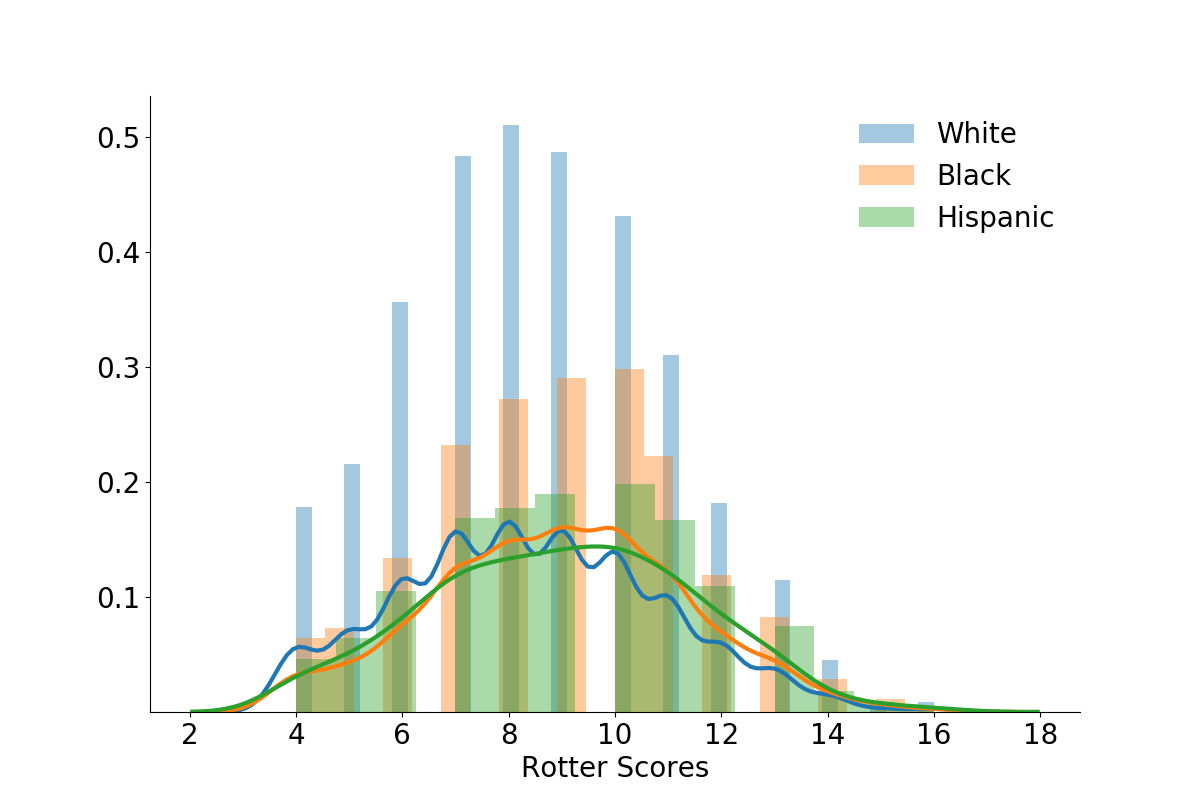
\includegraphics{fig-human-capital-race-rotter}}
\end{figure}\end{frame}
%-------------------------------------------------------------------------------
%-------------------------------------------------------------------------------
\begin{frame}\begin{figure}[htp]\centering
\caption{Rosenberg Score}
\scalebox{0.35}{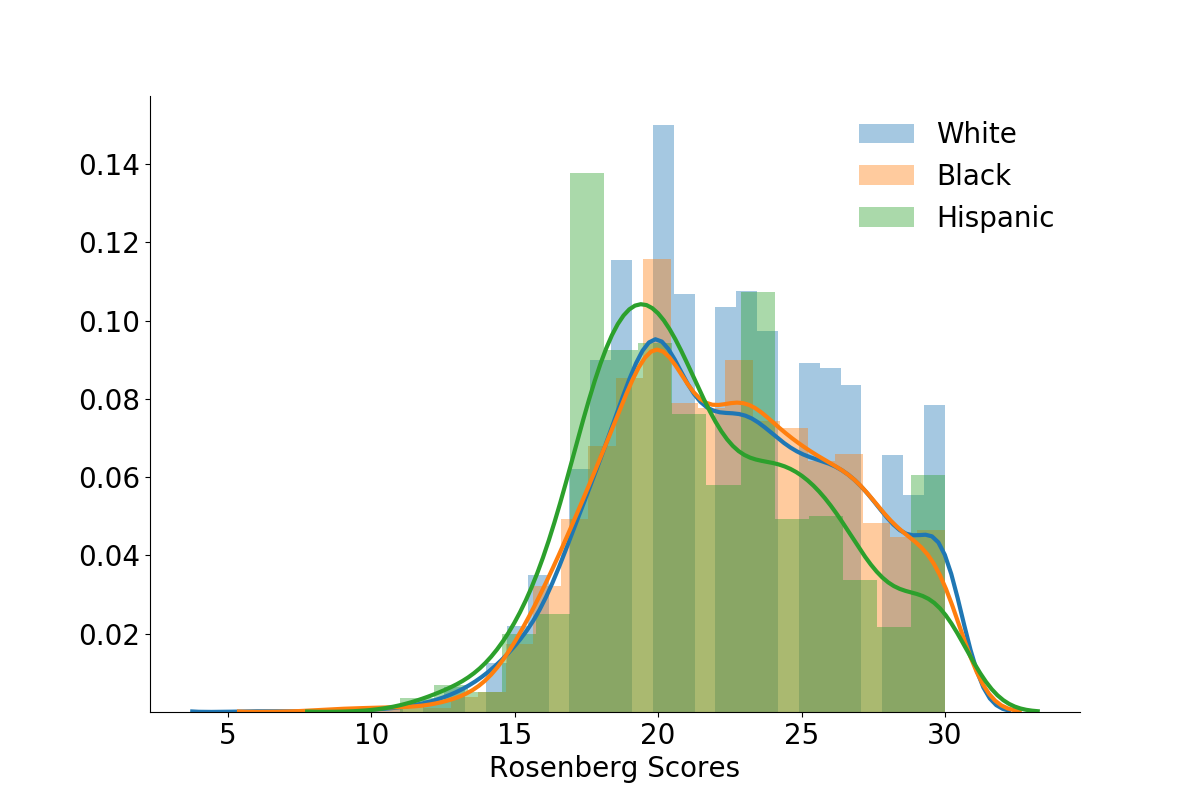
\includegraphics{fig-human-capital-race-rosenberg}}
\end{figure}\end{frame}
%-------------------------------------------------------------------------------
%-------------------------------------------------------------------------------
\begin{frame}\begin{center}
\LARGE\textit{Intergenerational Transmission}
\end{center}\end{frame}
%-------------------------------------------------------------------------------
%-------------------------------------------------------------------------------
\begin{frame}\begin{figure}[htp]\centering
\caption{Father's education}
\scalebox{0.35}{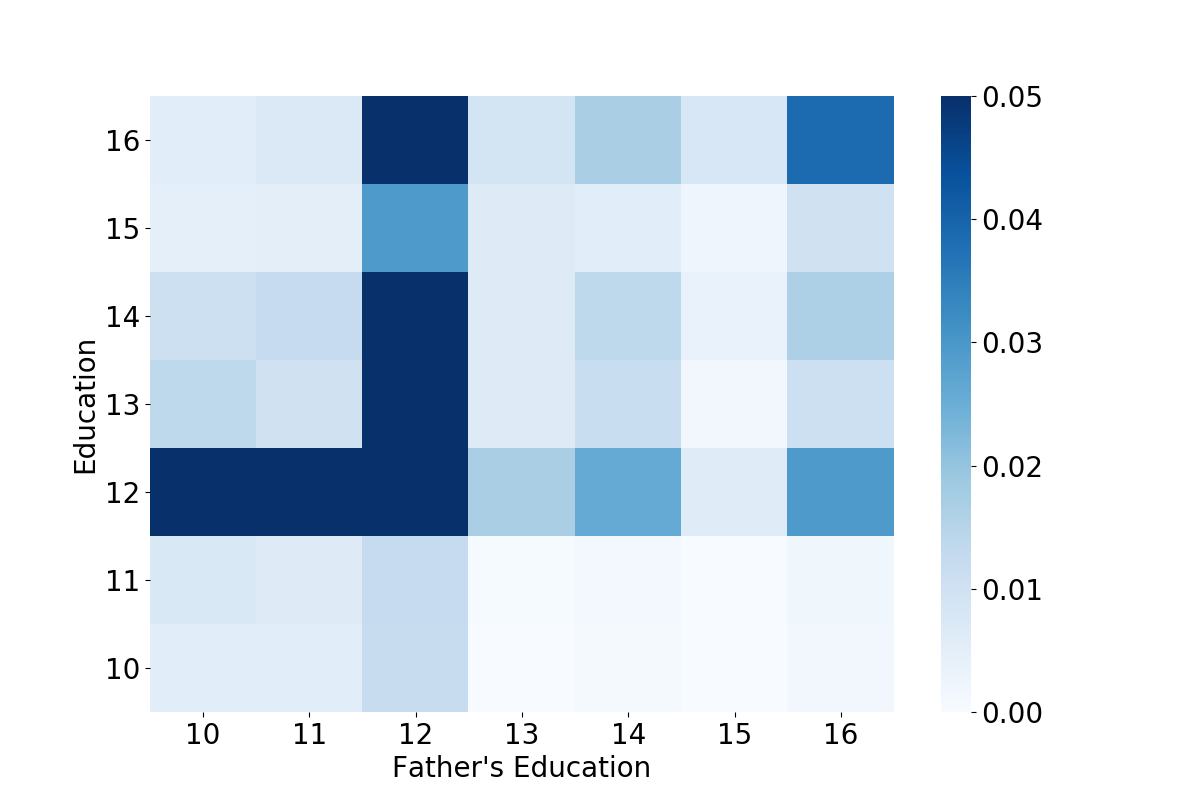
\includegraphics{fig-human-capital-intergenerational-father}}
\end{figure}\end{frame}
%-------------------------------------------------------------------------------
%-------------------------------------------------------------------------------
\begin{frame}\begin{figure}[htp]\centering
\caption{Mother's education}
\scalebox{0.35}{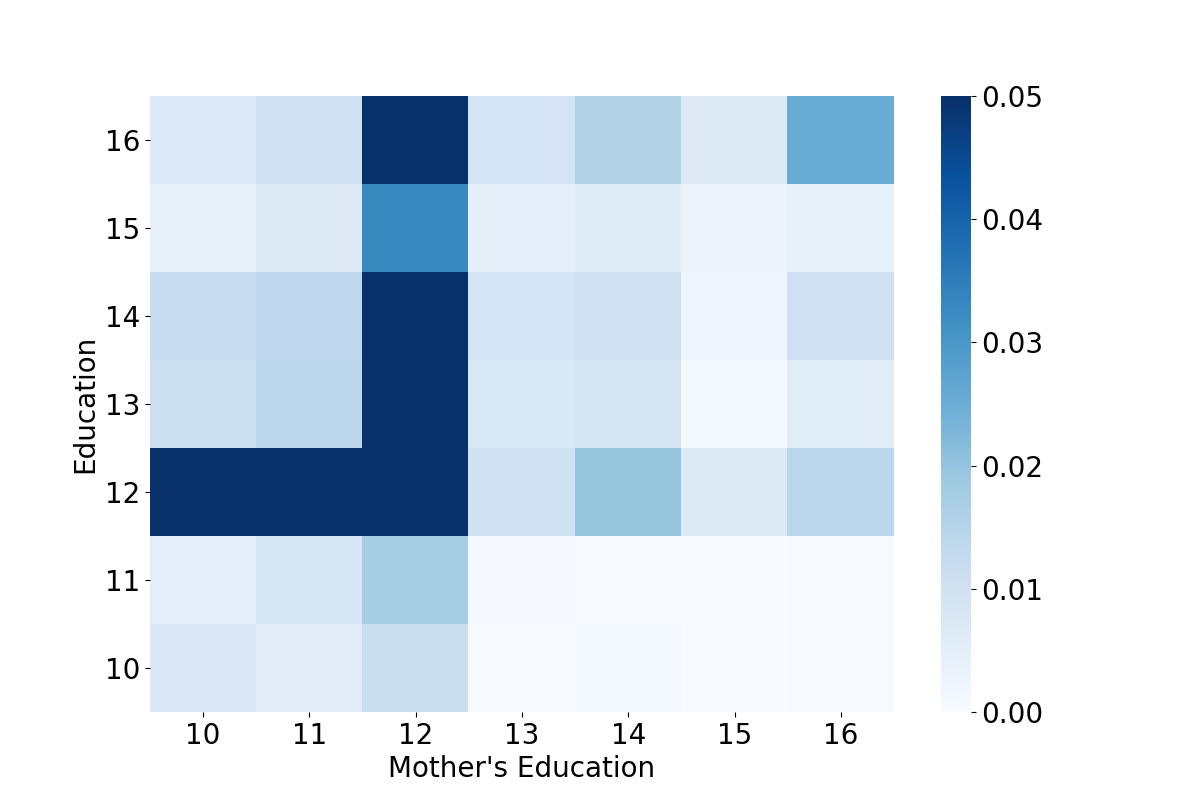
\includegraphics{fig-human-capital-intergenerational-mother}}
\end{figure}\end{frame}
%-------------------------------------------------------------------------------
%-------------------------------------------------------------------------------
